\documentclass[./main.tex]{subfiles}


\begin{document}
\chapter{Analisi Sperimentale}
% ------------- La libreria TPTP -------------
\section{La libreria TPTP}
\begin{figure}[h]
    \centering
    \scalebox{0.3}{
        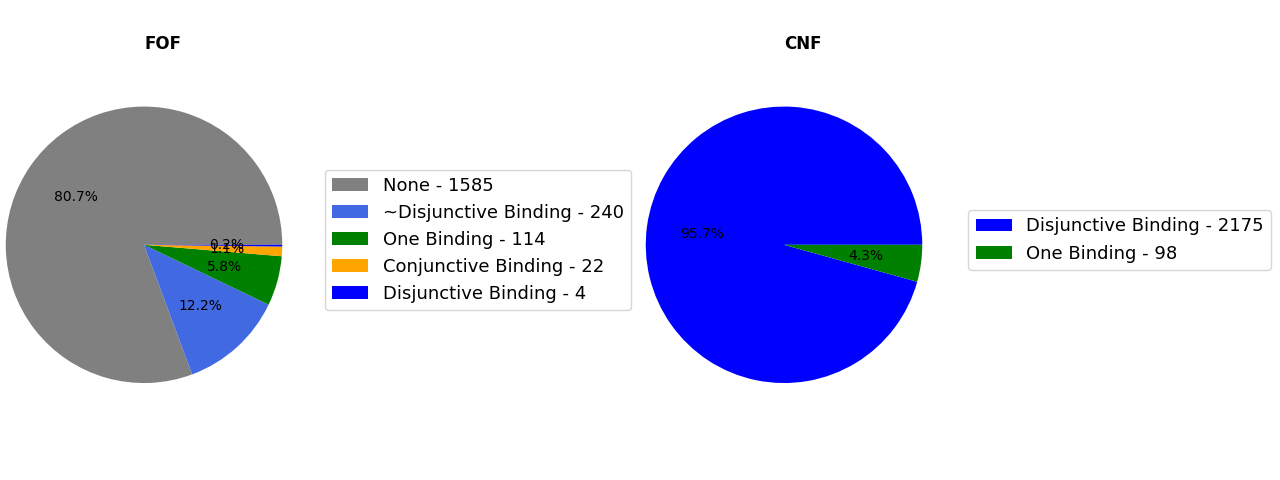
\includegraphics{images/5_sperimentazione/fof_cnf_classificazione.png}
    }
    \caption{Classificazione Libreria TPTP fof e cnf senza uguaglianza}
    \label{fig:classificazione_tptp}
\end{figure}

Per verificare la correttezza e l'efficienza dell'algoritmo implementato è stata scelta 
la libreria di problemi TPTP \cite{tptpLib} come dataset di problemi da risolvere. 
La libreria TPTP è una collezione di problemi per sistemi ATP dove ogni problema è scritto in formato
TPTP come descritto nella sezione \ref{sec:tptp_lang}.
I problemi TPTP sono suddivisi in base al dominio di appartenenza e al formato (fof, cnf, tff, ecc).
Il nome dei file segue il seguente schema:
\begin{verbatim}
    <domain><number>[+,-]<version>.p
\end{verbatim}

dove '$<$domain$>$' è il dominio di appartenenza del problema ed è composto da tre lettere maiuscole, mentre
'$<$number$>$' è un numero, generalmente di tre cifre, che identifica il problema all'interno del dominio.
Il simbolo + indica che il problema è scritto con la sintassi \textit{fof} mentre il simbolo - indica
che il problema è scritto con la sintassi \textit{cnf}. La stringa '$<$version$>$' è un suffisso che
identifica la versione del problema.
Ad esempio, un nome valido è \textit{SYN001+1.003.p}, che indica il problema 1 del dominio \textit{Syntactic},
in formato \textit{fof}, versione 1.003. 

Non tutti i problemi sono adatti per essere risolti con l'algoritmo implementato ed è 
stato, quindi, necessario filtrare i problemi in base a determinate caratteristiche.
In primo luogo, sono stati scartati tutti i problemi non in formato \textit{fof} o \textit{cnf} e
i problemi con uguaglianza. Questo è stato possibile tramite il comando \textit{TPTP2T}:

\begin{itemize}
    \item Per i problemi fof: \texttt{tptp2T -q2 -pps Form FOF -Equality}
    \item Per i problemi cnf: \texttt{tptp2T -q2 -pps Form CNF -Equality}
\end{itemize}

Il risultato delle due query ha restituito una lista di \textbf{1969} problemi in formato \textit{fof} e
\textbf{2274} problemi in formato \textit{cnf}. 
Da entrambe le liste è stato scartato un problema puramente proposizionale,
quindi poco significativo per la sperimentazione, ma estremamente grande da rallentare l'intero set di benchmark,
riducendo il numero di potenziali problemi utili a \textbf{1965} per i problemi \textit{fof} e \textbf{2273} per i problemi \textit{cnf}.

Successivamente, tutti i problemi sono stati classificati tramite il classificatore descritto nella sezione \ref{sec:classifier}.
Si ricorda che i problemi sono dati in formato $(A_1 \land A_2 \land ... \land A_n) \rightarrow C$, dove 
$A_1, A_2, ..., A_n$ sono assiomi e $C$ è la congettura, mentre 
sia l'algoritmo di decisione che Vampire lavorano sul problema negato, ovvero $A_1 \land A_2 \land ... \land A_n \land \lnot C$.
Per classificazione di un problema $P$ con congettura si intende, quindi, l'identificazione del frammento di appartenenza del problema negato $\lnot P$.
Nelle formule in cui non è presente la congettura, come quelle del formato \textit{cnf}, 
per classificazione della formula $P = A_1 \land ... \land A_n$ si intende l'identificazione del frammento di appartenenza del
problema non negato $P$.
I risultati della classificazione sono mostrati in figura \ref{fig:classificazione_tptp}.

Riguardo ai problemi \textit{fof}, dei \textbf{1965} problemi analizzati:
\begin{itemize}
    \item \textbf{1585} sono stati classificati come \textit{None} e quindi totalmente inutilizzabili.
    \item \textbf{114} sono \textit{One Binding} e \textbf{22} sono \textit{Conjunctive Binding}, quindi adatti per l'algoritmo.
    \item \textbf{244} sono \textit{Disjunctive Binding} e quindi non adatti per l'algoritmo.
\end{itemize}
Dei \textbf{244} problemi \textit{Disjunctive Binding}: \textbf{240} contengono la congettura mentre gli altri \textbf{4} non la contengono.
I \textbf{240} problemi con la congettura sono stati recuperati negandoli, in modo tale da portarli nel formato $\lnot A_1 \lor ... \lor \lnot A_n \lor C$, 
che fa parte del frammento \textit{Conjunctive Binding} e quindi adatto per l'algoritmo 
(questi problemi nella figura \ref{fig:classificazione_tptp} sono chiamati \textit{$\sim$Disjunctive Binding}).
Questo porta ad un numero totale di \textbf{376} problemi utili in formato \textit{fof}.

Riguardo ai problemi \textit{cnf}, la suddivisione è più netta.
Tutte le formule CNF sono infatti o del frammento \textit{One Binding}, se per ogni clausola
tutti i letterali della clausola hanno la stessa lista di termini, o altrimenti del frammento \textit{Disjunctive Binding}.
Dei \textbf{2273} problemi analizzati:
\begin{itemize}
    \item \textbf{98} sono del frammento \textit{One Binding}
    \item \textbf{2175} sono del frammento \textit{Disjunctive Binding}
\end{itemize}
In questo caso, la negazione delle formule \textit{Disjunctive Binding} porterebbe a problemi puramente proposizionali e quindi poco utili per la sperimentazione.
Il totale dei problemi utili in formato \textit{cnf} è quindi di \textbf{98}. Per un totale di \textbf{474} problemi utili.
La lista dei \textbf{474} problemi è riportata nell'appendice \ref{app:numerazione_problemi}.
Ogni problema è stato numerato nella tabella \ref{tab:numerazione_problemi} in appendice \ref{app:numerazione_problemi} per essere facilmente identificato.
% ------------- La libreria TPTP -------------


% ------------- Analisi dei risultati -------------
\section{Metodologia Sperimentale}
In questa sezione verranno analizzati i risultati dell'esecuzione dell'algoritmo sui problemi selezionati nel paragrafo precedente
e confrontati con i risultati ottenuti da Vampire. 
L'obbiettivo della sperimentazione è confrontare l'efficienza di un algoritmo gneral purpose basato su Resolution, come quello implementato da Vampire,
con un algoritmo specializzato SMT, come quello implementato nel capitolo \ref{chap:progettazione}.
Vampire implementa numerose strategie euristiche e inferenze di semplificazione per essere efficiente a livello competitivo.
Quindi, per indurlo a comportarsi il più possibile come il modello della \textit{Given Clause} descritta 
nella sezione \ref{sec:vampire_saturazione}, è stato necessario disabilitare/impostare alcune opzioni.
% In particolare sono state disattivate tutte le semplificazioni 
% e le euristiche applicabili ad entrambi gli approcci ma non presenti in modo comune alle attuali implementazioni.
L'algoritmo di saturazione adottato è stato \textit{Otter}, 
poiché l'algoritmo predefinito \textit{LRS} non offre garanzie di completezza e
si basa sull'uso di limiti di tempo e memoria come criteri di selezione/semplificazione, 
utilizzandoli come vero e proprio input che influenza il calcolo. 
È preferibile evitare questa metodologia, poiché si desidera che gli algoritmi confrontati abbiano quantomeno lo stesso input
e che non dipendano dai limiti di tempo e di memoria.
Per il \textit{preprocessing} sono state disabilitate tutte le semplificazioni non comuni a entrambi gli algoritmi.
In particolare, l'opzione \textit{-updr} (Unused Predicate Definition Removal) è stata disabilitata, in quanto non utilizzata dall'algoritmo
Binding. 
Come regola di semplificazione è stata disattivata l'opzione \textit{-fs} (Forward Subsumption) che elimina 
clausole che sono sussunte da altre clausole durante la fase di \textit{Forward simplification} 
(Una clausola $D$ è sussunta da una clausola $C$ se esiste una sostituzione $\sigma$ tale che 
$C^\sigma \subseteq D$, clausole del genere vengono cercate dalla $fs$ e rimosse perché ridondanti).
È stata disattivata anche l'opzione \textit{-av} (AVATAR - Advanced Vampire Architecture
for Theories and Resolution) che è un metodo SMT implementato in Vampire per lo splitting delle clausole tramite un Sat solver.
L'opzione \textit{-av} è stata disattivata dato che l'obbiettivo è quello di far utilizzare a Vampire solo calcoli del primo ordine.
Il comando utilizzato per l'esecuzione di Vampire è quindi il seguente:
{
\small    
\begin{verbatim}
    vampire --mode vampire -sa otter -t 10m -m 12000 -av off -updr off -fs off <problem>
\end{verbatim}}
Dove \textit{$<$problem$>$} è il problema da risolvere. 
Come limiti di tempo e memoria sono stati impostati rispettivamente 10 minuti e 12GB di ram.
L'algoritmo per i frammenti Binding è stato eseguito con i seguenti parametri:
{
\small    
\begin{verbatim}
    vampire --mode 1b -t 10m -m 12000 <problem>
\end{verbatim}}
I risultati riportati di seguito sono stati estrapolati dall'esecuzione del programma su un 
Macbook Pro 2018, 2.9 GHz 6-Core Intel Core i9, 16 GB 2400 MHz DDR4 sistema operativo macOS Sonoma 14.0.
Gli esperimenti sono stati poi ripetuti su un computer Windows 11 con processore Intel Core i9-13900K e ram 32GB DDR5
sul sottosistema Windows for Linux (WSL) e si sono ottenuti tempi di esecuzione, come da aspettativa, più bassi ma assolutamente coerenti,
mentre per memoria i valori sono rimasti esattamente gli stessi.
I tempi delle tabelle si riferiscono ai tempi rilevati dalla macro $Time\_Trace$ posta all'inizio dell'algoritmo per i frammenti Binding 
e all'inizio del \textit{MainLoop} di Vampire escludendo quindi i tempi di parsing e preprocessing.
Per una maggior accuratezza, i tempi sono stati calcolati come media di 5 esecuzioni.
Le tabelle delle misurazioni di tempo e memoria sono riportate nell'appendice \ref{app:tabelle_misurazioni}.

\section{Analisi dei Risultati}
\subsubsection{One Binding}

% -------- fof 1b naif
\grafico{images/5_sperimentazione/time/1b/fof_1b_naif.png}{Tempo Vampire vs 1b naif, problemi fof del frammento One Binding}{fig:fof_1b_naif}
\grafico{images/5_sperimentazione/time/1b/fof_1b_naif_compresso.png}{Tempo Vampire vs 1b naif, problemi fof del frammento One Binding. Grafico limitato a 40 ms.}{fig:fof_1b_naif_compresso}

Partendo dai problemi \textit{fof} del frammento \textit{One Binding} è possibile osservare un grafico in figura \ref{fig:fof_1b_naif}
relativo alla tabella \ref{tab:fof_1b_time} dell'appendice \ref{app:tabelle_misurazioni} dei tempi di esecuzione (Vampire in color rosso sangue e l'algoritmo naif color foglia di tè). 
Si nota subito che, nonostante la maggior parte dei problemi venga risolta in tempi molto brevi da entrambi, 
nell'ordine di millisecondi, l'algoritmo naif si comporta molto bene rispetto a Vampire.
Questo anche perché molti dei problemi selezionati sono risultati puramente proposizionali e, quindi, risolti direttamente dal SAT solver
senza la necessità di richiamare l'algoritmo effettivo.
Nella tabella questi problemi sono contrassegnati con una '(g)' a fianco tempo.
È noto, infatti, che per problemi proposizionali i SAT solver sono molto più efficienti rispetto ad algoritmi per la logica del primo ordine.
I problemi risolti in pochi millisecondi e i problemi proposizionali sono poco significativi per il confronto.
Nell'intero set di Benchmark vi sono, però, tre problemi non proposizionali interessanti. 
In particolare, i problemi di KRS (Knowledge Representation): 7, 21 e 25.
In tutti e tre i problemi Vampire va in timeout (10 minuti).
Nel problema 7 anche l'algoritmo naif raggiunge i limiti di timeout,
mentre il problema 21 viene risolto in 5 millisecondi e il problema 25 in meno di un millisecondo.
Il problema 7 è l'unico dei One Binding fof che mette in difficoltà l'algoritmo naif.
Analizzando le statistiche del problema, si nota che il $99\%$ del tempo viene impiegato dalla ricerca 
dei mus. 
Andando a vedere come è formato, si scopre che il problema è composto da tanti $\tau$-Binding 
molto semplici che però hanno tutti lo stesso termine più qualche termine ground con termini diversi.
Il problema crea tanti nuovi BindingLiterals uguali, $b_1(x_1), ..., b_2(x_n)$, che fanno esplodere la ricerca del mus non ottimizzato.

Sulla memoria non c'è molto da dire, entrambi gli algoritmi utilizzano in media $400Kb$, tranne nei casi
dei problemi proposizionali in cui Vampire ne consuma molta di più. 
L'unico caso più interessante è sempre il problema 7, in cui Vampire utilizza circa $10Gb$, 
arrivando quasi al limite (12Gb) e l'algoritmo naif ne utilizza meno di $1Gb$.
Questo vuol dire che, probabilmente, anche avendo a disposizione più tempo Vampire non avrebbe comunque concluso le verifiche
per mancanza di memoria, mentre l'algoritmo naif avrebbe potuto continuare ancora per molto.

\grafico{images/5_sperimentazione/mem/1b/fof_naif_mem.png}{Memoria Vampire vs 1b naif, problemi fof del frammento One Binding}{fig:fof_1b_naif_mem}

% -------- cnf 1b naif
\grafico{images/5_sperimentazione/time/1b/cnf_1b_naif.png}{Tempo Vampire vs 1b naif, problemi cnf del frammento One Binding}{fig:cnf_1b_naif}
\grafico{images/5_sperimentazione/time/1b/cnf_1b_naif_compresso.png}{Tempo Vampire vs 1b naif, problemi cnf del frammento One Binding. Grafico limitato a 80 ms.}{fig:cnf_1b_naif_compresso}

Anche per i problemi \textit{cnf} del frammento \textit{One Binding} si possono fare le stesse osservazioni fatte sopra.
Nella figura \ref{fig:cnf_1b_naif} si può osservare il grafico dei tempi di esecuzione estratto dalla tabella \ref{tab:cnf_1b_time} dell'appendice \ref{app:tabelle_misurazioni}.
Molti dei problemi cnf non sono altro che la conversione dei rispettivi problemi fof ed è, quindi, ragionevole
che i tempi di esecuzione siano simili.
Anche qui vi sono tre casi interessanti. 
I due problemi 457 e 461 del dominio SYN (Syntactic) e il problema 408 del dominio PUZ (Puzzle). 
Anche in questo contesto Vampire, raggiunge il limite di timeout in tutti e tre i problemi.
Nel problema 408 anche l'algoritmo naif raggiunge il limite di timeout.
Nei problemi 457 e 461 l'algoritmo naif risolve il problema rispettivamente in circa 6 e 9 millisecondi.
Anche per questo problema il $99\%$ del tempo per la risoluzione del problema 408 è impiegato nella ricerca dei mus.
Il problema non ha alcuna caratteristica rilevante, se non che ha un'alta concentrazione di letterali ground.
Riguardo alla memoria, anche in questo caso entrambi si mantengono in media sui $400Kb$ tranne nei casi già discussi in precedenza.


% -------- fof 1b ottimizzato
\grafico{images/5_sperimentazione/time/1b/fof_1b.png}{Tempo Vampire vs 1b, problemi fof del frammento One Binding}{fig:fof_1b}

% Simulando l'esecuzione dell'algoritmo mus naif su un input del tipo $b_1(t), ..., b_2(t)$, dove i 
% $b_i$ sono BindingLiterals e $t$ è un termine comune, succede questo:
% \begin{itemize}
%     \item Viene effettuata la prima chiamata su $b_1(t)$ e si cercano i letterali unificanti.
%     Il primo letterale, che restituisce il SubstitutionTree è $b_1(t)$ (questo dipende anche dall'ordine di inserimento).
%     Il letterale $b_1(t)$ fa già parte della soluzione e quindi si passa al prossimo letterale.
%     Il letterale successivo è $b_2(t)$ e si aggiunge alla soluzione.
%     \item Viene effettuata la seconda chiamata ricorsiva su $b_2(t)^\sigma$ dove $\sigma$ è l'unificatore
%     di $b1$ e $b2$ cioè la sostituzione vuota. Quindi la chiamata ricorsiva viene effettuata su $b_2(t)$.
%     \item Viene creato un nuovo iteratore sul SubstitutionTree che restituisce in ordine 
%     $b_1$ e $b_2$ che vengono scartati perché già presenti nella soluzione.
%     In generale ad ogni livello con input $b_x$ vengono scartati $x$ letterali per trovare un nuovo
%     letterale da aggiungere alla soluzione.
%     \item Il ciclo si ripete finchè non si arriva a $b_n$ e si è trovato il mus.
% \end{itemize}
% Tutto ciò accade solo nel primo ramo dell'albero di ricorsione.
% In un input del genere è facile vedere che il mus è unico ed è composto da tutti i letterali,
% ma l'algoritmo naif una volta terminata la chiamata, ad esempio su $b_1$, il letterale viene bloccato
% e viene cercato il mus che contiene il letterale successivo, in questo caso $b_2$, senza considerare il letterale bloccato ($b_1$).
% È evidente che viene fatto molto lavoro inutile.
% La strategia adottata per ottimizzare questa ricerca è stata quella di verificare se la sostituzione $\sigma$ è vuota.
% Nel caso della chiamata su $b_1$, la sostituzione con $b_2$ è vuota quindi si aggiunge $b_2$ alla soluzione e si 
% continua ad iterare sul SubstitutionTree senza effettuare la chiamata ricorsiva.
% Il risultato finale è l'algoritmo \ref{alg:mus} spiegato nel capitolo precedente.
Analizzando l'algoritmo naif si nota che il caso peggiore, cioè quello che porta a $O(2^n)$ chiamate ricorsive,
 si verifica quando si ha un input del tipo $b_1(t_1), ..., b_1(t_n)$,
dove $t_1, ..., t_n$ sono termini tutti unificabili. 
Il problema 7 è proprio un'istanza di questo caso. 
L'ottimizzazione introdotta per aggirare questi casi 
è stata quella di verificare la composizione della sostituzione proposta dal SubstitutionTree.
Nel caso in cui la sostituzione sia vuota, si prosegue con l'esplorazione del SubstitutionTree senza effettuare chiamate ricorsive.
L'implementazione è spiegata nel dettaglio nel capitolo precedente.

Questa ottimizzazione ha portato un miglioramento in tutti i problemi One Binding fof e cnf, e, come si vedrà in seguito, 
anche negli altri frammenti. 
Anche solo con questa ottimizzazione è stato possibile risolvere i problemi 7 e 408.
La seconda ottimizzazione è stata l'aggiunta dell'algoritmo \ref{alg:groundMus} groundMus 
in combinazione con l'ordinamento dell'insieme di implicanti.
Ordinando gli implicanti in modo da avere per primi i letterali ground, si induce l'algoritmo a ricercare per 
primi i mus dei letterali ground, che sono più semplici da trovare.
Ordinando invece gli implicanti in modo da far stare vicini i letterali con termini uguali, si induce 
l'algoritmo a utilizzare la prima ottimizzazione.
% Il suo funzionamento e le sue motivazioni e funzionamento sono spiegate nel capitolo precedente.
L'ottimizzazione del groundMus è l'ottimizzazione più significativa che è stata introdotta, in termini di risparmio di tempo e memoria.
È da precisare che, comunque, i tempi di esecuzione erano già molto bassi prima delle ottimizzazioni,
quindi sarebbe da verificare il loro reale impatto su problemi più complessi.
Di seguito sono mostrati i grafici dei tempi di esecuzione di Vampire e dell'algoritmo ottimizzato.


% -------- cnf 1b
\grafico{images/5_sperimentazione/time/1b/cnf_1b.png}{Tempo Vampire vs 1b, problemi cnf del frammento One Binding}{fig:cnf_1b}

\subsubsection{Conjunctive Binding}
\grafico{images/5_sperimentazione/time/cb/cb_time.png}{Tempo Vampire vs 1b naif, problemi fof del frammento Conjunctive Binding}{fig:fof_1b_conj}
La maggior parte dei problemi del frammento \textit{Conjunctive Binding} sono risolti in meno di un millisecondo sia da Vampire che dall'algoritmo naif.
Gli unici casi interessanti sono il problema 135 e 136 del dominio SYO (Syntactic).
L'esecuzione del programma sul problema 135 raggiunge la soglia di timeout sia per Vampire che per l'algoritmo naif 
e usano rispettivamente 10Gb e 1Gb di memoria.
Nel problema 136, invece, l'algoritmo naif raggiunge la soglia di timeout e Vampire lo risolve in appena 400 millisecondi, 
utilizzando rispettivamente 1Gb e 4Mb di memoria.
La prima ottimizzazione è stata sufficiente per risolvere il problema 135 in 200 millisecondi.
Con l'aggiunta dell'ottimizzazione groundMus, il problema 135 viene risolto in 120 millisecondi.
Il problema 136 invece non viene risolto nei limiti di tempo nemmeno con l'aggiunta delle due ottimizzazioni.
Il problema 136 è un teorema, ciò significa che la sua negazione è insoddisfacibile.
L'algoritmo deve, quindi, dimostrare che ogni insieme di implicanti trovato dal Sat solver è insoddisfacibile.
Analizzando le statistiche, si è visto che anche se, grazie all'ottimizzazione groundMus,
per ogni insieme di implicanti veniva trovata una contraddizione in tempi ragionevoli, 
ogni nuovo modello proposto dal Sat solver differiva dal precedente per il valore di pochi letterali.
Il modo in cui si è diminuito il numero di assegnamenti da verificare è stato quello di utilizzare 
l'ultimo mus trovato per generare la clausola bloccante. 
Dato un insieme $I$ di letterali
e un suo sottoinsieme $U \subseteq I$, si può dimostrare facilmente che, se la congiunzione dei letterali
di $U$ è insoddisfacibile, allora lo è anche la congiunzione dei letterali di $I$.
In gergo, questo insieme di letterali insoddisfacibile è detto \textit{unsat core}.
Si può notare che l'ultimo mus trovato è proprio un unsat core dell'insieme di implicanti, anche se non è detto che sia il più piccolo.
Con questa terza ottimizzazione in combinazione con le altre due, il problema 136 viene risolto in circa 6 secondi utilizzando 20Mb di memoria.
Nell'intero set di Benchmark, questo è l'unico problema che, 
in termini di tempo e memoria, si discosta così tanto da Vampire.


\subsubsection{Disjunctive Binding}
\graficoDb{images/5_sperimentazione/time/db/db_naif.png}{Tempo Vampire vs 1b naif, problemi fof del frammento Disjunctive Binding}{fig:fof_1b_disj}

Nei problemi di Disjunctive Binding negati, emerge un chiaro svantaggio dell'algoritmo naif rispetto alla soluzione offerta da Vampire. 
Anche con l'applicazione delle ottimizzazioni, si registra un miglioramento, 
ma non al punto da poter competere con la velocità di Vampire. È da notare che, 
nonostante i tempi di esecuzione inefficienti dell'algoritmo naif, 
il consumo di memoria rimane inferiore.

\graficoDb{images/5_sperimentazione/mem/db/db_naif_mem.png}{Memoria Vampire vs 1b naif, problemi fof del frammento Disjunctive Binding}{fig:fof_1b_disj}

Considerato che, nell'algoritmo naif, le uniche operazioni dispendiose in termini di 
memoria sono la generazione di clausole e la ricerca dei mus, si 
è ipotizzato che questo ridotto utilizzo di memoria sia dovuto al fatto che
l'albero di ricorsione dell'algoritmo mus sia molto basso.
Uno dei motivi per cui può capitare questa situazione è che il problema contenga 
una prevalenza di letterali ground.
L'ipotesi è stata confermata analizzando le statistiche dei problemi e
si è visto che il Sat solver in alcuni casi restituiva un insieme di implicanti
composto esclusivamente da letterali ground.
Di conseguenza, l'algoritmo verificava inutilmente la soddisfacibilità dell'insieme trovato,
rifacendo in modo estremamente meno efficiente ciò che in realtà era già stato fatto dal Sat solver.
Per ovviare a questo problema, è stato aggiunto un controllo che verifica se l'insieme di implicanti 
è composto esclusivamente da letterali ground e, in tal caso, si restituisce direttamente $\top$.
I problemi Disjunctive sono gli unici che presentano questa caratteristica e questo è 
dovuto soprattutto al fatto che sono stati generati della negazione dei problemi originali.
In una formula del tipo $\lnot A_1 \lor ... \lor \lnot A_n \lor C$ è sufficiente che una delle 
formule tra gli assiomi e la congettura sia ground affinché 
sia possibile avere un insieme di implicanti ground.
Nel grafico \ref{fig:fof_1b_disj_ott} è possibile osservare come quest'ultima 
ottimizzazione abbia migliorato i tempi di esecuzione,
rivelando, però, che anche in questo caso i problemi verificati sono poco significativi.
Anche qui, nella tabella \ref{tab:fof_db_time} i problemi che fanno uso di questa ottimizzazione sono contrassegnati con una '(g)' a fianco del tempo.

\graficoDb{images/5_sperimentazione/time/db/db.png}{Tempo Vampire vs 1b, problemi fof del frammento Disjunctive Binding}{fig:fof_1b_disj_ott}


\section{Conclusioni e Possibili Sviluppi futuri}
Nonostante i problemi analizzati si siano rilevati poco significativi, 
i risultati ottenuti sono comunque interessanti e rivelano le potenzialità dell'algoritmo.
La sperimentazione ha inoltre riconfermato la netta superiorità dei Sat solver o più in generale di sistemi 
basati su SMT rispetto ad algoritmi puramente basati su Resolution per la risoluzione di problemi proposizionali.
Guardando tutto l'insieme dei risultati si nota che l'algoritmo ottimizzato è in grado di risolvere più problemi rispetto a Vampire 
e in generale 'vince' in termini di tempo e memoria per la maggior parte dei problemi.
Se si considerano il tempo totale per l'esecuzione dei benchmark si vede che l'algoritmo naif impiega circa 1 ora 
mentre Vampire impiega circa 4.5 ore e l'algoritmo ottimizzato impiega solo 15.6 secondi.
Questi tempi così alti sono dovuti ovviamente ai timeout.
Considerando i problemi comuni risolti sia da Vampire e l'algoritmo naif si vede che l'algoritmo naif impiega
circa 19.5 minuti mentre Vampire impiega solo 4.8 minuti. 
Questo distacco è dovuto principalmente ai problemi Disjunctive. 
Se non si considerano i problemi Disjunctive, l'algoritmo naif impiega infatti circa 400 millisecondi contro i 4.3 minuti di Vampire.
Il conteggio totale delle vittorie è di 337 a 109 in favore dell'algoritmo naif.
Se non si considerano i problemi puramente ground le vittorie dell'algoritmo naif scendono a 273 contro 109 di Vampire.
Passando invece all'algoritmo ottimizzato, se si considerano solo i problemi risolti sia da Vampire che dall'algoritmo ottimizzato,
Vampire impiega 4.8 minuti mentre l'algoritmo ottimizzato impiega 15.6 secondi.
Se si escludono tutti i problemi puramente ground e i problemi Disjunctive risolti con la quarta ottimizzazione,
il totale è di 5 secondi per Vampire e 5.9 secondi per l'algoritmo ottimizzato.
Di questi 5.9 secondi però, 5.8 sono impiegati per risolvere il problema 136 cioè il $98\%$ del tempo totale.  
Se non si considera questo problema l'algoritmo ottimizzato impiega 0.1 secondi contro i 4.9 secondi di Vampire.
Il conteggio delle vittorie è di 426 a 21 in favore dell'algoritmo ottimizzato. 
Se si escludono i problemi ground e i problemi risolti con la quarta ottimizzazione, il conteggio scende a 150 a 21.

A parte il problema 136, la differenza di tempo tra Vampire e l'algoritmo ottimizzato è davvero minima, nell'ordine di 
decimi di millisecondi e non è quindi possibile stabilire quale approccio sia migliore per problemi non proposizionali.
Il set di benchmark andrebbe ampliato con problemi più complessi per effettuare un confronto più significativo.
Anche generando dei problemi più specifici per il frammento.
Moti dei problemi selezionati infatti fanno parte del frammento Bernays–Schönfinkel, quindi senza funzioni, oppure
spesso contengono solo predicati unari o binari.
Sarebbe interessante anche effettuare un confronto con altri theorem prover come IProver e E.

Il primo passo da compiere per migliorare l'algoritmo è quella di modificare la procedura di preprocessing.
Modificando le funzioni standard di Vampire per la trasformazione in CNF e il Namig si
eliminerebbe la necessità di creare i \textit{booleanBinding} arrivando anche a dimezzare il numero di letterali creati.
Andrebbe anche studiata la semplificazione updr (Unused definitions and pure predicate removal) e 
applicata, se possibile, al preprocessing.
Andando ad utilizzare direttamente il Sat solver senza passare dall'interfaccia di Vampire 
si potrebbero sfruttarne appieno le potenzialità. 
Ad esempio, in questa implementazione quando viene trovato un mus, viene creato un Sat solver da zero e inizializzato con tutte le Sat clausole associate ai letterali del mus.
Questo comporta un notevole dispendio di tempo. 
Una strategia alternativa sarebbe quella di aggiungere le clausole del mus nel corso della visita dell'albero di ricorsione 
e eliminarle quando non più necessarie. 
Al momento, nell'interfaccia di Vampire è possibile solo aggiungere clausole ma non rimuoverle ed 
è per questo che l'algoritmo non è stato implementato in questo modo fin da subito.
Per quanto riguarda il problema 136, il motivo per cui Vampire impiega così poco tempo 
è attribuibile alle euristiche di selezione delle clausole. 
Andrebbe indagato se e quali euristiche possono essere applicate anche all'algoritmo implementato per guidarne l'esecuzione.
L'ottimizzazione groundMus è stata l'euristica più significativa che ha permesso di risolvere la maggior parte dei problemi
che l'algoritmo naif non riusciva a risolvere.
% Se una formula contiene molti letterali ground, allora è probabile che portino ad una contraddizione.
% Se invece non ne contiene o ne contiene pochi il groundMus dovrebbe terminare comunque in tempi ragionevoli.
Il problema che così com'è implementato il sorting degli implicanti, l'ordine di priorità di selezione dei letterali ground è dato esclusivamente da come 
viene data in input la formula. 
Una strategia sarebbe quella di dare un ordine di priorità in base al numero di volte che un letterale ground compare
con polarità opposta in una Sat clausola per massimizzare la probabilità di trovare una contraddizione.
Con questa strategia probabilmente si riuscirebbe a risolvere il problema 136 in tempi più ragionevoli.
Questa analisi non dovrebbe essere molto diversa da quella fatta da updr.
Un altro aspetto del preprocessing è che non è escluso che vi siano dei LiteralBinding ground.
Questo accade perché i booleanBinding vengono creati prima della skolemizzazione mentre i LiteralBinding vengono creati dopo.
Si potrebbe aggiungere un'opzione per scomporre i LiteralBinding ground una volta skolemizzati 
o comunque aggiungere un controllo del tipo che se la sotto formula ha un prefisso esistenziale con polarità positiva (o universale con polarità negativa) allora non crea il booleanBinding.
Seguendo questa strada però bisognerebbe aggiungere uno step in più per skolemizzare la FBE e 
inoltre verificare che il Naming non causi problemi.
Non è stato indagato su come questo aspetto possa impattare sulle prestazioni dell'algoritmo.
Da un lato la creazione di questi booleanBinding semplifica il lavoro del Sat solver durante la ricerca dell'implicante,
dall'altro però, potrebbe appesantire il lavoro che viene fatto all'interno dell'algoritmo.
Inoltre questo aspetto potrebbe andare in conflitto con l'ottimizzazione proposta in precedenza per il groundMus.
Un altro aspetto critico da migliorare, sempre riguardo la ricerca dei mus, è la ricerca dei letterali unificanti all'interno del SubstitutionTree.
In particolare, andrebbe creato un iteratore ad hoc per navigare il SubstitutionTree.
In questa implementazione ad ogni livello viene creato un nuovo iteratore che spesso propone letterali già presenti nella soluzione
facendo molto lavoro di unificazione inutile.

In conclusione, l'approccio proposto si è dimostrato promettente e vi sono molte strade da esplorare 
per migliorare l'algoritmo e renderlo più competitivo, 
tuttavia, sono richieste ulteriori indagini e sviluppi per formulare conclusioni definitive su quale sia l'approccio migliore.







\end{document}